Ever since ancient Greece people have been trying to discover what makes up everything. Back then they said that everything was comprised of four elements: earth, fire, water, and air. Although modern scientists use a few more than four elements, they are still trying to categorize the most fundamental element that makes up everything. Democritus, an ancient Greek scientist, proposed that everything if divided enough times could be broken down into atoms their most fundamental object. While some people names something the atom that was not the most fundamental substance, scientists today are still pursuing the "atom" theorized by Democritus, the most fundamental substance. 

In the 19th century John Dalton believed he found the most fundamental particle and named it the atom, but as time passed there was very strong evidence that even atoms had internal components and structure. This was proven when J.~J.~Thompson in the late 19th century found the electron, which ended up being a component of the atom. This was not only the first fundamental particle discovered, but also the beginning of particle physics as a field of study. While it was an insightful discovery that led to many inventions, there were still many unknown things about the atom. About a decade after Thompson, Robert Millikan made fine measurements of the charge and mass of the electron, but this raised many questions about the atom. It was not until Ernest Rutherford in the early 20th century showed that the atom is mostly empty space with a very dense core called the nucleus which has an opposite charge to that of the electron. He did this by shooting alpha particles, made up of two protons and two neutrons, at gold foil and observing their in scattering angle. In this experiment most of the alpha particles passed through unperturbed while a handful were majorly deflected. From this observation, Rutherford made the conclusion most of the atom was empty space while having a highly dense core called the nucleus. 

These discoveries showed there were more things to explore past the atom, and in parallel there were equally important theories being developed. Quantum mechanics is essential to the study of sub-atomic particles as they no longer behave according to classical mechanics. During this time Max Planck was doing his work on the quantization of energy. This set the ground work for quantum mechanics and also served as a basis to Einstein's work. In 1905 Einstein formulated his theory of special relativity, which had several major impacts on the field of particle physics. One of the major ones was quantization of light into particles called photons. Although light had long been thought of as a wave Einstein showed many of its particle-like properties leading to the wave-particle duality of light. Eventually De Brogile extended this duality to all particles theorizing that all particles including electrons and other sub-atomic particles could be described using waves or particles.

Einstein's theory of relativity had another major impact on particle physics. Probably the most famous of Einstein's equation, $E = mc^2$, shows the mass-energy relationship. One of the implications of quantum mechanics is that if something can happen it will happen under a certain probability. This means that given the right conditions and enough energy one can simply create mass. There are other conservation laws that need to be followed that are still relevant to particle physics, but conservation of energy is one of the biggest limiters as it says to create more massive particles more energy is needed. 

As these theories became more complete, they allowed for the further description of sub-atomic particles, like the states of the electrons in the atoms and the protons and neutrons that make up the nucleus of the atom. Scientist also began to find evidence of fundamental particles not in atoms. In 1932 Carl Anderson found evidence of a muon from cosmic rays. In addition, as scientists began to probe higher energies they found evidence of internal structure within protons and neutrons. In 1968 at the Standford Linear Accelerator Center they found evidence of particles within protons and neutrons, which were later called quarks.

The discovery of more and more fundamental particles led to the formulation of the standard model. Part of the standard model included something like a periodic table for fundamental particle. The two main groups of particles on the standard model are fermions, which have half integer spin and bosons, which have integer spin. The main physical difference this causes is from the Pauli exclusion principle, which allows fermions to build into larger arrangements. Because of this fermions are the building blocks of the macroscopic world as they make up protons neutrons, and atoms.   

As shown in table~\ref{tab:particles} there are several different groups of particles in the standard model. The first group is a sub-category of fermions called quarks. The main thing that distinguishes quarks from other fundamental fermions is that they interact via the strong force. While they also interact via the electromagnetic and weak force the strong force is the more dominate one. Quarks can exist in isolation only for a short time, but rather exist in groups of two three or possibly more. When three quarks form a particle it is called a baryon. A proton which is made up of two up and one down quarks and a neutron which is made up of two down and one up quarks are baryons. Each of the quarks inside a baryon has a different color red, green, or blue which serves as the "charge" for the strong force. Like electric charge strong force color attracts other colors and repels similar, but since the baryon has one of each it has a net color of white or nothing. In addition to the six flavors of quark listed on table~\ref{tab:particles} there is also a corresponding anti-quark with the same properties except for opposite charge and color. Quarks can also form in pairs called mesons, which have a quark and anti-quark. If one tries to separate the individual quarks from the respective baryons or mesons the energy required to separate them is more than the energy required to simply create more quarks. If one tries to separate a proton into its constituent quarks the necessary input energy would rather create new quarks forming baryons and mesons leaving no quark in isolation. 

The other category of fermionic particles are the leptons. Unlike the quarks, leptons are not affected by the strong force so it is more common to find them in isolation. The electron is the most well-known lepton but there are also two other flavors which are heavier copies of the electron. As with all of the particles on the standard model there are corresponding anti-particles for the each lepton with the same mass but opposite charge. In addition to the three charged leptons there are also three neutral leptons which are called neutrino. Each one has a charged lepton pair. Neutrinos are nearly mass-less and do not have any charge. Since the only force that affects them is the weak force they have a very low probability of interaction. This means that they essentially pass through everything without interaction. Although they do interact through processes like beta decay most neutrinos simply just go through everything. 

Finally, there are the bosons. Bosons are different from both leptons and quarks in that they have integer spin, but the individual bosons differ in which fundamental force affects them. While leptons and quarks combine together to form complex arrangements such as atoms and all of matter, bosons serve as the force carriers. The photon serves as the mediator for the electromagnetic force. This means that whenever two electrons repel each other there is a photon to mediate that interaction. The strong force interaction is mediated by the gluon. The weak force is mediated by the W boson, for those interactions with changes in charge and Z bosons for those interaction with no changes in charge. 

\begin{table}
\caption{Particles on the Standard Model}
\label{tab:particles}
\begin{center}
\begin{tabular}{|c|c|c|c|c|}
\hline
Particle Type & Name & Charge & Mass & Spin \\
\hline
\multirow{6}{*}{Quarks} & Up & $+2/3$ & $2.2\MeVcc$ & $\pm 1/2$ \\
& Down & $-1/3$ & $4.7\MeVcc$ & $\pm 1/2$ \\
& Charm & $+2/3$ & $1.28\GeVcc$ & $\pm 1/2$ \\
& Strange & $-1/3$ & $96\MeVcc$ & $\pm 1/2$ \\
& Top & $+2/3$ & $173.1\GeVcc$ & $\pm 1/2$ \\
& Bottom & $-1/3$ & $4.18\GeVcc$ & $\pm 1/2$ \\
\hline
\multirow{6}{*}{Leptons} & Electron & $-1$ & $0.511\MeVcc$ & $\pm 1/2$ \\
& Muon & $-1$ & $105.7\MeVcc$ & $\pm 1/2$ \\
& Tau & $-1$ & $1.776\GeVcc$ & $\pm 1/2$ \\
& Electron Neutrino & $0$ & $\approx 0$ & $\pm 1/2$ \\
& Muon Neutrino & $0$ & $\approx 0$ & $\pm 1/2$ \\
& Tau Neutrino & $0$ & $\approx 0$ & $\pm 1/2$ \\
\hline
\multirow{4}{*}{Gauge Bosons} & Photon & 0 & 0 & $\pm 1$ \\
& Gluon & 0 & 0 & $\pm 1$ \\
& W boson & $\pm 1$ & $80.4\GeVcc$ & $\pm 1$ \\
& Z boson & 0 & $91.19\GeVcc$ & $\pm 1$ \\
\hline
Scalar Boson & Higgs Boson & 0 & $125.1\GeVcc$ & 0 \\
\hline
\end{tabular}
\end{center}
\end{table} 
One nice thing about the standard model is that it gives this very convenient table of fundamental particles but discovery all of these particles was not simple. The electron is the only particle in the standard model that is found in isolation at energies used on earth. To find the next particle, the muon, scientist had to look at cosmic rays, which provided the energy needed to create these particles. While neutrinos are plentiful they interact so infrequently scientist are still struggling to create an efficient detector for them. To discover the remaining particles in the standard model they had to use particle colliders. Throughout the last few decades, scientists have built colliders to probe higher and higher energies, to make them capable of discovering more fundamental particles. In 2012, using the Large Hadron Collider at CERN scientists were able to find evidence of the Higgs boson, the final particle in the standard model. However, there are still phenomenon in the universe that cannot be explained using the standard model, such as gravity and dark matter. There are several theories beyond the standard model that offer explanations for these, but they also say there are more fundamental particles to be discovered at higher energies. This is one of the main goals of the LHC experiment. 

% Add a figure related to the Higgs discovery? or recent plot summarizing various Higgs property measurements?
\begin{figure}
\centering
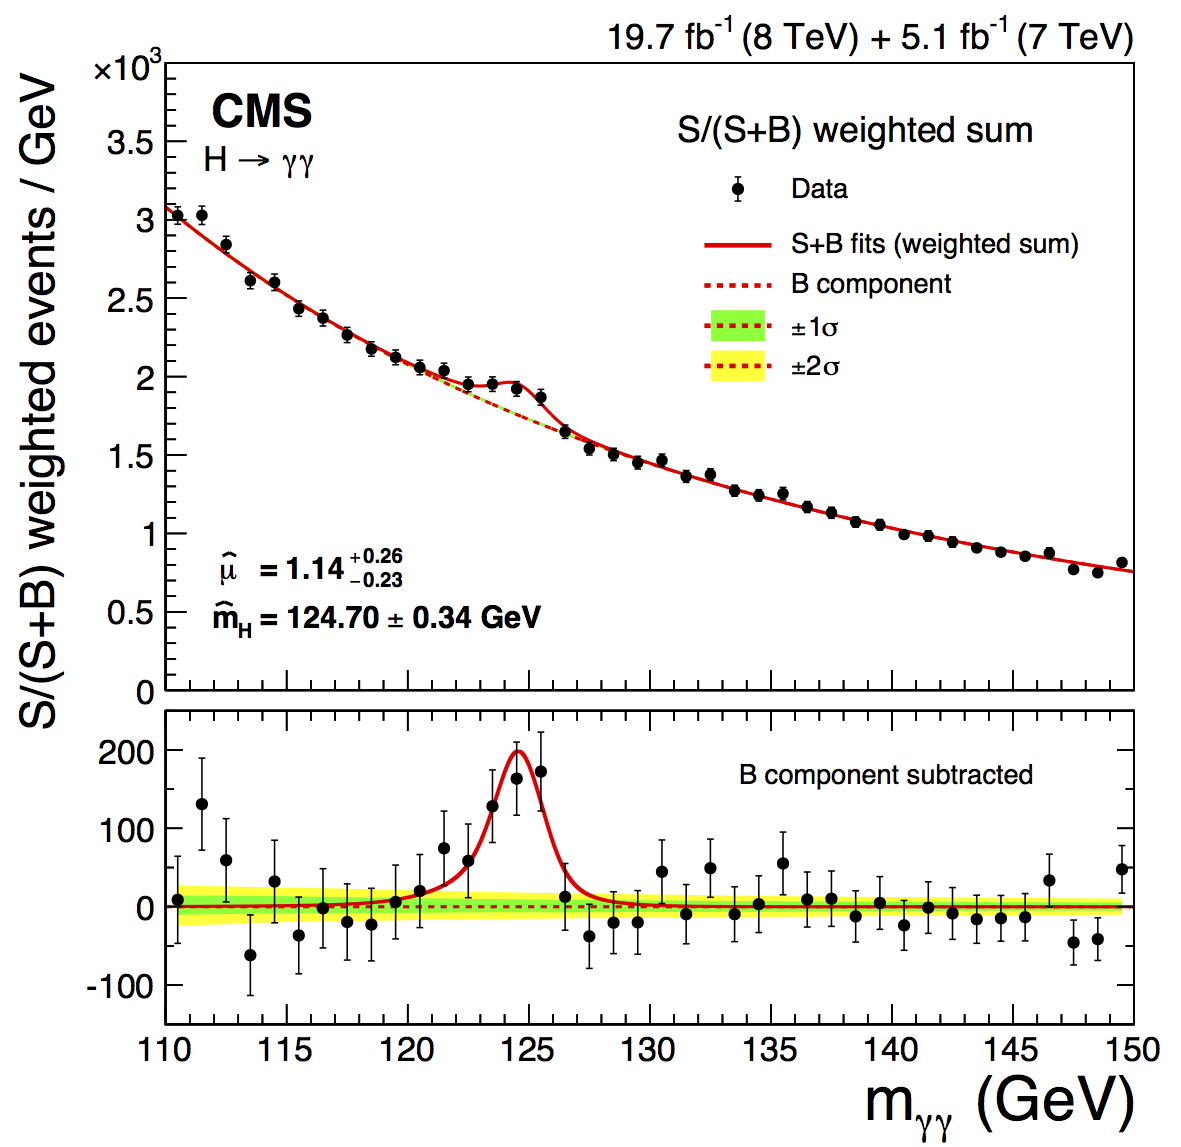
\includegraphics[width=0.6\linewidth]{Figures/higgsmeasurement.png}
\caption{Data showing evidence of the Higgs Boson from a two photon decay.}
\label{fig:higgs}
\end{figure} 

Fermions and quarks are the building blocks of all of matter. All of the atoms on the periodic table are made up of electrons, and up and down quarks, which make up protons and neutrons. Aside from the neutrinos, the particles in higher generations are extremely similar to the respective particle in the first generation except for being a substantially higher mass. Because of this these particles have very short lifetimes and are only found in high energy interactions. For instance, when cosmic rays hit the earth's atmosphere they provide the energy to create muons. To find the particles like the top quark, which is over 1000 times more massive than the muon, the colliders need to collide particles together at even higher energies. The LHC at CERN, is the highest energy collider humans have built to date and has started searching for particles at energies previously not achieved. One of the detectors on the LHC is the Compact Muon solenoid, which is the detector I worked on during my undergraduate career at Baylor. Chapter~\ref{chap:LHC_CMS} will discuss the details of the LHC and CMS detector as more specific background to my work. 